%% -*- fill-column: 120; -*-
\section{PoET: Proof of Elapsed Time}
\label{sec_poet}


At the beginning of each consensus round, a validator builds a block that extends the chain it believes to be the
correct one (note that the selection of a chain to extend is an implicit ``vote'' for the chain). Next, the validator
performs a computation that determines a time duration it must wait before it may claim leadership and extend the chain
with the block it constructed. If no one claims leadership before the time expires, the validator broadcasts
its proposed block and a proof that it computed the time correctly. The chain is extended with the new block and the
process begins again. 

The future time that is computed represents a form of ``lottery'' where every validator is given a ticket and the
validator with the smallest ticket wins the lottery. The computation used to generate the lottery ticket must meet
several important criteria:

To provide resiliency to Byzantine faults:
\begin{itemize}
\item Censorship Resistant
  The computation should distribute leader election across the broadest possible population of participants. Fairness
  ensures that no single validator can persistently control the transactions that may be committed; that is, fairness
  ensures censorship resistence.

\item Sybil Prevention
  The cost of controlling the leader election process should be proportional to the value gained from it. Investment
  limits the potential for an organization to control consensus by ``flooding'' the process with voters without a
  corresponding investment of resources. Investment democratizes consensus. 
\end{itemize}

To ensure efficient execution:
\begin{itemize}
\item Distribute Wait Times
  The communicatio nefficiency of Nakamoto consensus is a result of implicit voting and 

\item Simplify Verification
  While the cost of computing the lottery function should be high to ensure investment, it should be relatively simple
  for all participants to verify that the function was performed correctly. This asymetry in computation ensures that
  false leadership claims can be identified quickly and rejected.

\item Adapt to Changing Populations

\end{itemize}




Nakamoto consensus involves an uncoordinated, distributed leader election.

Leader election must be easily verifiable.
This is efficient if the leader can be established with a single broadcast. 

Nakamoto consensus is efficient when all validators accept a leader with a single broadcast.
Distributed in time such that a single node believes it is at the front of the line and has time to communicate that
fact to all other nodes before any other node believes it is at the front of the line.

\begin{center}
  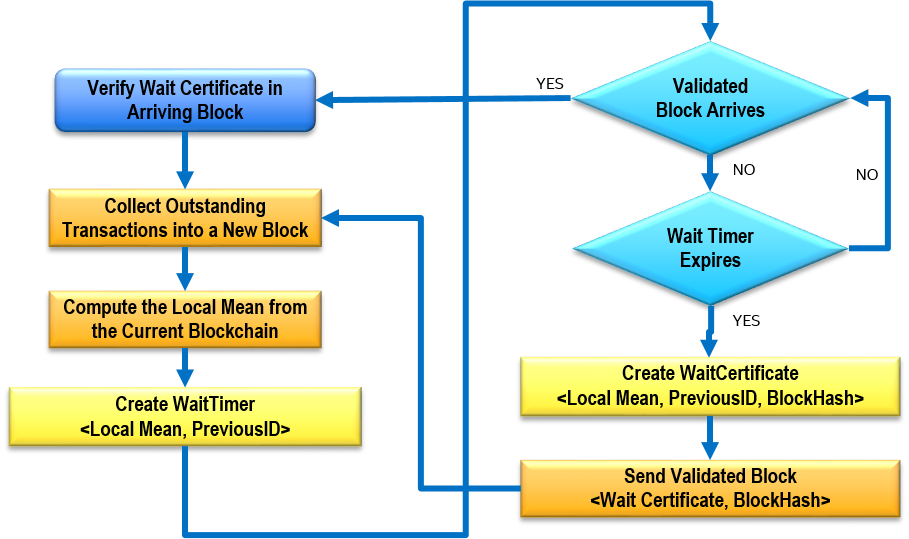
\includegraphics[scale=.75]{figures/PoET_Flow.png} \
  \caption{Control flow in the PoET protocol}
  \label{fig:poetflow}
\end{center}

\subsection{Local Mean Computation}

\subsection{Fork Resolution}

